%%%%%%%%%%%%%%%%%%%%%%%%%%%%%%%%%%%%%%%%%%%%%%%%%%%%%%%%%%%%%%%%%%%%%
%% Start the main part of the manuscript here.
%%%%%%%%%%%%%%%%%%%%%%%%%%%%%%%%%%%%%%%%%%%%%%%%%%%%%%%%%%%%%%%%%%%%%
\section{Introduction}

Protein-protein interactions underlie many biological processes, including signal transduction and antibody-antigen recognition.
In fact, mutations at protein-protein interfaces are over-represented within disease-causing mutations\cite{jubb_mutations_2017}, indicating the central importance of these interactions to biology and impications to human health.
A computational method capable of predicting mutations that strengthen or weaken known protein-protein interactions would not only serve as a useful experimental tool to improve our understanding of biology, but would also enhance our ability to create protein drugs with new methods of actions, and additionally enhance engineering applications such as design of protein-based sensors and materials.

Several prior methods have attempted to predict changes in binding free energies using different approaches to scoring and sampling,
including weighted energy functions that set to describe physical interactions underlying protein-protein interactions\cite{guerois_predicting_2002,kamisetty_accounting_2011},
statistical and contact potentials \cite{dehouck_beatmusic:_2013,moal_intermolecular_2013,vangone_contacts-based_2015,brender_prediction_2015},
a combination of these approaches\cite{li_predicting_2014},
graph-based representations\cite{pires_mcsm:_2014},
and methods that attempt to sample backbone structure space locally around mutations\cite{dourado_multiscale_2014}.

We set out to develop and assess methods for prediction of change in binding free energy after mutation (interface \ddg) within the Rosetta macromolecular modeling suite. Rosetta is freely available for academic usage, allowing future combination of these predictions with Rosetta's powerful protein design capabilities, which has proven successful in a variety of applications (TODO cite Rosetta reviews only)\cite{kaufmann_practically_2010}.
Prior projects have applied Rosetta predictions to
dissect determinants of binding specificity and promiscuity (TODO REF 14527405, 12679019),
enhance protein-protein binding affinities \cite{sammond_structure-based_2007}, TODO add REF 16354667
and to design modified (TODO REF 15034550, 22403064)  and new interactions (TODO REFs 12419232 Sarel), but no prior benchmarking effort has studied the performance of predicting changes in binding free energy in Rosetta on a large, diverse benchmark data set, in part because such a dataset has only become available more recently.
The current state-of-the-art Rosetta \ddg\ method,  ddg\_monomer \cite{kellogg_role_2011}, has proven effective at predicting changes in stability in monomeric proteins after mutation, but had not yet been tested at predicting change of binding free energies in protein-protein complexes.
Prior ``computational alanine scanning'' \ddg\ methods were benchmarked on mutations in protein-protein interfaces, focusing on mutations to alanine \cite{kortemme_simple_2002,kortemme_computational_2004,conchuir_web_2015}.
This alanine scanning method sampled only side chain degrees of freedom, which is a fair approximation for mutations to alanine (which are not expected to cause large backbone perturbations\cite{cunningham_high-resolution_1989}), but a less probable assumption for mutations to larger side chains which might require some degree of backbone rearrangement to accommodate the change.
Adaptation of this alanine scanning method to recent score function and sampling method developments in Rosetta has not shown improvement in benchmarking\cite{conchuir_web_2015}, indicating a need to more thoroughly develop and test a method that attempts to more aggressively sample conformational space.

We sought to create a method that would take into account the natural conformational flexibility of proteins by representing structures as an ensemble of individual full-atom models, generating sufficient microstate-like models to effectively explor the biologically relevant and accessible portions of conformational space close to the native structure.
Ensemble representations have proven their effectiveness to predict change in protein stabilities after mutation\cite{benedix_predicting_2009} and to improve $\Delta G_{binding}$ calculations between kinases and their inhibitors \cite{araki_effect_2016}.

We chose to sample conformational diversity through use of the ``backrub'' protocol implemented in Rosetta.
The backrub method samples using local, coupled, side chain and backbone motions, similar to those observed in high-resolution crystal structures \cite{davis_backrub_2006}.
Backrub ensembles appears to recapitulate properties of proteins that have been experimentally determined, such as side chain NMR order parameters\cite{friedland_simple_2008}, sequence profiles at protein-protein interfaces \cite{humphris_prediction_2008}, sequence profiles of protein-peptide binding specificity \cite{smith_structure-based_2010,smith_predicting_2011}, and can sample the conformational variability between protein homologs\cite{schenkelberg_protein_2016}.
Backrub has also proved effective in design applications, such as for the redesign of protein-protein interfaces (TODO REF 22403064) and recapitulation of mutations that alter ligand-binding specificity\cite{ollikainen_coupling_2015}.
When Davey and Chica compared backrub ensembles to ensembles generated via molecular dynamics simulations or PertMin, backrub ensembles were shown in certain cases to be
``the only ensemble which has a diversity that is greater than its average deviation from crystal structure, a consequence of the ability of Backrub motions to mimic high resolution dynamics from solution NMR while maintaining structural similarity to the input crystal structure''.\cite{davey_improving_2014}
We hypothesized that this property of backrub ensembles would translate into these ensembles serving as an effective structural representation to use when predicting interface \ddg\ values.

\section{Methods}

Developing and testing with confidence a new method to predict changes in binding free energy after mutation requires a large benchmark set of covering single mutations, multiple mutations, mutations to all amino acid types, and mutations across a variety of complexes.
Skempi \cite{moal_skempi:_2012} is the largest known database of known \ddg s in protein-protein interfaces, but can be curated further for maximum effectiveness for method development and benchmarking.
In part to prevent overfitting our method on a benchmark set of our own creation, we have chosen to use a dataset created by Dourado and Flores\cite{dourado_multiscale_2014} during the creation of their ZEMu (Zone Equilibration of Mutants) method.
The ZEMu dataset was curated for effectiveness in benchmarking an interface \ddg\ method, including filtering SKEMPI values derived from non-peer reviewed data.
Confidence in the ``known'' experimental \ddg\ values is important, as it has been shown that the experimental methodology used can have a strong effect on the performance of predictors of changes in binding free energy\cite{geng_exploring_2016}.
The ZEMu dataset was also curated to include a wide range of both stabilizing and destabilizing mutants, small side chain to large side chain mutations, single and multiple mutations, and a diversity of complexes (\cref{tab:table-composition}).

\subimport*{figs-and-tables/}{table-composition}

After a review of the literature from which the known experimental \ddg\ values originated, we removed one data point from the 1254 point ZEMu set that we could not match to the originally published reported affinity value. We also removed 5 mutations we determined to be duplicates, along with 8 mutations that were reverse mutations of other data points, leaving us with a test set of 1240 mutations.
We defined which complexes that contained at least one antibody binding partner by comparison of PDB identifiers with SAbDab \cite{dunbar_sabdab:_2014}.

Our protocol, called ``flex ddG'', is implemented within the RosettaScripts scripting interface to the Rosetta macromolecular modeling software suite \cite{fleishman_rosettascripts:_2011}, which makes the protocol easily adaptable to future improvements and energy function development. We utilized Rosetta's Talaris \cite{leaver-fay_chapter_2013,song_structure-guided_2011,shapovalov_smoothed_2011} energy function.
Version numbers of tested software are available in \cref{tab:table-versions}.

\begin{figure}
  \centering
  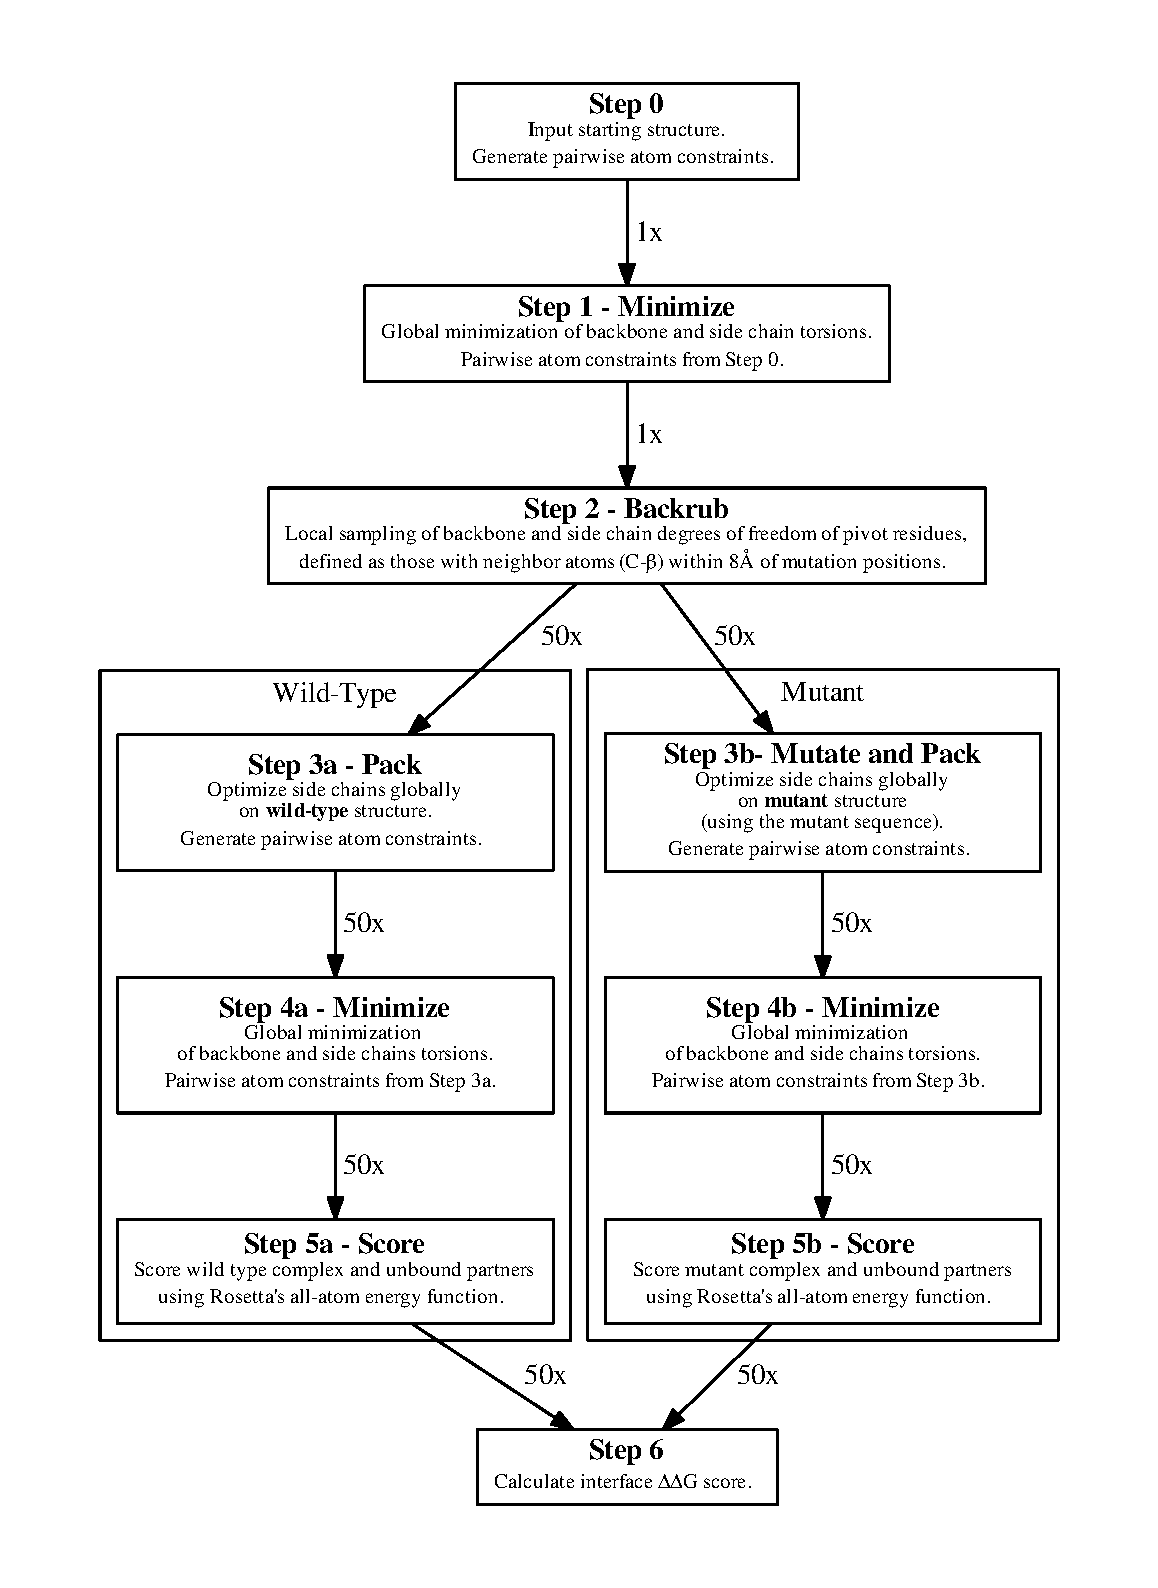
\includegraphics[width=\textwidth,keepaspectratio]{figures/fig-overview.pdf}
    \caption{
      Schematic of the flex ddG protocol method.
  } \label{fig:figure-overview}
\end{figure}

Flex ddG method steps are outlined in \cref{fig:figure-overview}.
Step 1: The protocol begins with an initial minimization to calibrate the input model to the Rosetta energy function. This (and later) minimizations are performed with constraints that harmonically restrain pairwise atom distance to their values in the input crystal structure.
Step 2: The backrub method is run, at a temperature of 1.2, for up to 60,000 backrub Monte Carlo trials. 50 output structures are generated, which will be used as the base of conformational diversity for the rest of the week.
Step 3A: For each of the 50 structure models in the ensemble (output by backrub), the Rosetta ``packer'' is run to search side chain space through the Dunbrack rotamer library built into Rosetta\cite{shapovalov_smoothed_2011}, optimizing side chains for the wild type sequence.
Step 3B: Independently and in parallel to step 3A, the packer is run on the 50 backrub models, optimizing side chains for the mutant sequence. Step 4A: Minimization of each of the 50 wild-type structures, again adding pairwise atom-atom constraints to the input structure.
Step 4B: Minimization of each of the 50 mutant structures.
Step 5A: Each of the 50 minimized wild-type structures are scored in complex, and the individual complex components are scored individually. The scores of the split, unbound complex components are obtained simply by splitting the complex halves away from each other. No further minimization or side chain optimization is performed on the unbound states before scoring.
% Note: I have tested repacking the unbound state (as per ALF's suggestion), and it gives worse performance
Step 5B: In the same fasion as Step 5A, each of the 50 minimized mutant structures are scored in complex, and the individual complex components are scored individually. Step 6: The interface ddG score is produced via Eq. \ref{eqn:split-ddg}:

\begin{equation}\label{eqn:split-ddg}
  \begin{split}
    {\Delta\Delta}G_{bind} & ={\Delta}G^{MUT}_{bind} - {\Delta}G^{WT}_{bind}\\
    & =({\Delta}G^{MUT}_{complex} - {\Delta}G^{MUT}_{partner A} - {\Delta}G^{MUT}_{partner B})\\
    & \quad - ({\Delta}G^{WT}_{complex} - {\Delta}G^{WT}_{partner A} - {\Delta}G^{WT}_{partner B})\\
  \end{split}
\end{equation}

We evaluate performance of the protocol by comparing predicted ddG scores to known experimental values, using Pearson's correlation R, MAE, and Fraction Correct (FC). Fraction Correct is defined as the number of mutations categorized as stabilizing, neutral, or destabilizing correctly, divided by the total number of mutations in the benchmark set. Stabilizing mutations are defined as those with a \ddg\ $<=$\ -1.0 kcal/mol, neutral as those with -1.0 kcal/mol $<$\ \ddg\ $<$\ 1.0 kcal/mol, and destabilizing as those with \ddg\ $>=$\ 1.0 kcal/mol.

MAE (Mean Absolute Error) is defined in Eq.~\ref{eqn:mae} as:

\begin{equation}\label{eqn:mae}
  MAE = \dfrac{1}{n}\sum\limits_{i=1}^n|y_i-x_i| = \dfrac{1}{n}\sum\limits_{i=1}^n|e_i|
\end{equation}

where $y_i$ are the predicted \ddg\ values, $x_i$ are the known, experimentally determined values, and $e_i$ is the prediction error.

\section{Results and discussion}

\subimport*{figs-and-tables/}{table-main}

Main performance of the protocol is summarized in \cref{tab:table-main}. Performance is shown for 4 prediction methods: (a) our flex ddG backrub ensemble method, (b) the prior state-of-the-art Rosetta methodology, ddg\_monomer \cite{kellogg_role_2011}, (c) a control version of our flex ddG protocol which omits the backrub ensemble generation step, leaving only the minimization and packing steps, and (d) the ZEMu (zone equilibration of mutants) method\cite{dourado_multiscale_2014}.

Our flex ddG method outperforms the comparison methods on the complete dataset in each of the correlation, MAE, and fraction correct methods. On the small-to-large subset of mutations where we expect to see the largest performance gains from using a backbone ensemble method, we see a substantial improvement in performance as compared to the alternative methods.
Performance of the flex ddG on the subset of single mutations to alanine is also competitive or outperforms the alternative methods.
As we we do not expect single mutations to alanine to require intensive backbone sampling, as mutations to alanine can accommodate much of ramachandran space\cite{cunningham_high-resolution_1989}, our method's effectiveness on this subset shows that it is somewhat robust to the mutation type.
This can be explained by the fact that we undertake backrub sampling prior to making the mutation, helping ensure that we are sampling underlying, relevant flexibility of the input crystal structure, instead of distorting the local structure around a mutation to resolve a clash or poor interaction with a mutant side chain.
Finally, our method shows improved performance compared to the control method and ddg\_monomer on the subset of multiple mutations, but does not match the performance of the ZEMu method.
This could indicate that further refinement to the backrub sampling parameters are required in the case of multiple mutations, since because there are more mutation sites, there will be more surrounding backrub pivot residue sites.
However, flex-ddG outperforms ZEMu on multiple mutations if none of the mutations are to alanine (\cref{tab:table-mult}).

The underlying scatterplots for the flex ddG and control methods on the complete dataset and small-to-large subsets are shown in \cref{fig:figure-scatter}. Scatterplots for the underlying data behind the rest of the rows in \cref{tab:table-main} is shown in the Supplementary Information.

\subimport*{figs-and-tables/}{figure-scatter}

\subimport*{figs-and-tables/}{structs-v-corr-WildTypeComplex-zemu-12-60000-rscript-validated-t14}

\subsection{Effect of averaging more structures}

\cref{fig:structs-v-corr-WildTypeComplex-zemu-12-60000-rscript-validated-t14} shows the effect on performance as scores from an increasing number of wild type and mutant structures are averaged.
The structures used are first sorted by the score of the score of the corresponding repacked and minimized wild type structure, such that producing a \ddg\ with 1 structure will only the lowest (best) scoring structure, 2 structures will use the 2 lowest scoring structures, and so forth.
\cref{fig:structs-v-corr-WildTypeComplex-zemu-12-60000-rscript-validated-t14}(a) shows perfomance on the complete dataset.
As more structures, of increasingly high wild type complex score, are averaged, correlation with known experimental values increases.
Conversely, performance for the no backrub control method (shown in light blue) decreases as more structures are average.
This result indicates that sampling with backrub adds information that improves \ddg\ calculation, and adds it in such a way that cannot be quantified through score alone, as the additional structures being averaged have higher scores \cref{fig:wildtypecomplex-scores-complete}, and would traditionally be though of as being less predictive.

The ddg\_monomer method also sees an increase in performance on the complete dataset as more output structures are averaged (\cref{fig:structs-v-corr-WildTypeComplex-ddg-monomer-16-003-zemu-2}), indicating that ramping the repulsive term of the energy function during minimization in ddg\_monomer is likely to improve results by sampling conformational space more broadly.

Averaging across more structures show an even stronger positive effect on correlation \cref{fig:structs-v-corr-WildTypeComplex-zemu-12-60000-rscript-validated-t14}(b) for the subset of small-to-large mutations.
However, the subset of multiple mutations (where none are mutations to alanine) shown in \cref{fig:structs-v-corr-WildTypeComplex-zemu-12-60000-rscript-validated-t14}(c) does not see monotonically increasing performance as more structures are averaged, indicating that more parameterization of the backrub method might be necessary for multiple mutations.

The improved performance effect is also present in \cref{fig:structs-v-corr-WildTypeComplex-zemu-12-60000-rscript-validated-t14}(d) for the subset of single mutations to alanines, a subset where it is not expected that increased sampling is neccessary, indicating that increased sampling, in the very least, is not harmful for this case.

As it is not possible to select 20 best-scoring structures without first generating a n ensemble of 50 structures, and as the performance when choosing structures sorted in this fashion is not significantly improved over the results in \cref{fig:structs-v-corr-id-zemu-12-60000-rscript-validated-t14} (where there is no sorting of structures by score), simply generating 20-30 structures should constitute sufficient sampling for most use cases.

\subsection{Effect of changing backrub sampling steps}

Sampling can also be controlled by changing the length of the backrub simulation, as measured in the number of Monte Carlo sampling steps.
\cref{fig:steps-v-corr} shows the performance effect of increasing backrub simulation length (while averaging all 50 structures at each output step).
\ddg\ scores are calculated every 2,500 backrub steps (shown in circles for correlation and in squares for MAE).
A ``X'' marks the performance with zero backrub steps (control minimization and side chain packing only method).

As we also observed when measuring increased sampling by averaging over more structures, increased performance is seen in both correlation with experimental data and MAE as backrub simulation length increases, for the subset cases of small-to-large muations (panel b) and multiple mutations, none to alanine (panel c).
Performance gains are maximized at 30,000 backrub steps, after that point, performance is relatively flat.
Performance improves for the first step of 2500 backrub steps on the complete dataset and for single mutations to alanine, but remains relatively flat afterwards.

The increased performance seen is not simply a result of scores decreasing as the simulation progresses, as the score of the minimized wild type complex does not decrease uniformly across the sampled ensemble as the simulation progresses (\cref{fig:wildtypecomplex-scores-complete}).
\cref{fig:t14-mean-ensemble} shows that pairwise backrub ensemble RMSDs continue to increase throughout the backrub simulation for all subsets, indicating that dimishing returns at 30,000+ steps is not a result of failure to sample new states, but rather might indicate that sampling is simply ``sufficient'' at 30,000 steps to capture the necessary local change in structure that might occur post-mutation.

Unlike when increasing the number of averaged structures, we see continual improved performance with additional sampling (from longer backrub simulations) on the subset of multiple mutations (not to alanine). This indicates that the effects of increasing sampling through creating more structure models and running longer backrub simulations are not equivalent, and that both sampling parameters are important to consider when running the flex ddG protocol.

\subsection{Score analysis}

As the sampling/scoring problems of protein modeling are inextricably linked, it is often the case that improving one removes a constraint on the other, allowing for further improvements to be made on the other.
We desired to evaluate what performance improvements we could gain in interface \ddg\ prediction by reweighting the Rosetta energy function, which is weighted and parameterized for broad application, to this specific benchmark case.
Additionally, analyzing a reweighted energy function on a score term by score term basis could provide insight into which terms might benefit from future reparameterization, and which score terms are most predictive for our dataset.

We chose to reweight the energy function using a non-linear reweighting scheme similar to Generalized Additive Models (GAMs)\cite{wood_fast_2011}.
In this reweighting method, we use Monte Carlo sampling to fit either a linear transformation or a sigmoid function to the individual distributions of score terms, with the overarching goal of reducing the error between our predictions and known experimental values over the entire dataset.

As we do not modify our models of the unbound state, any effects on stability of the complex partners will cancel out, as the $\Delta G$\ of folding score of the unbound partners is subtracted from the total score of the complex (\ref{eqn:split-ddg}).
Not modeling conformational change in the unbound models might be effective because to modeling any such fluctuation might produce more noise than signal than noise when the scores for the bound and unbound states are subtracted.
This is supported by the prior observation that the mobility of amino acids at dimeric interfaces is generally lower than for other amino acids at the protein surface exposed to solvent \cite{zen_comparing_2010}.

The terms in the Rosetta Talaris energy function that cancel out to zero are: yhh\_planarity, pro\_close, hbond\_sr\_bb, ref, fa\_dun, fa\_intra\_rep, omega, p\_aa\_pp, and rama.
Seven score terms are left; combined they become the final interface \ddg\ score: fa\_sol, hbond\_sc, hbond\_bb\_sc, fa\_rep, fa\_elec, hbond\_lr\_bb and fa\_atr.

The fit sigmoid and linear functions are shown in \cref{fig:t14-fits-feats}.
The effect on the distribution of predictions is shown in \cref{fig:t14-fit-scatter}.

\section{Conclusions}

We have shown that our novel ``flex ddG'' method for predicting change in binding free energy after mutation in protein-protein interfaces is more effective than previous methods on a curated benchmark dataset.
Particular improvement in performance is seen on the subset of small-to-large mutations, indicating that modeling backbone flexibility does improve performance on this case where post-mutation backbone rearrangements are expected to be more common.

We have also shown more accurate predictions can be obtaining by averaging the scores across a generated ensemble of backrub microstates, and that the number of required states is relatively low (20-30).
Prior methods that attempted to produce \ddg\ predictions by averaging an ensemble of models required orders of magnitude more structures  \cite{benedix_predicting_2009}, indicating that backrub sampling can efficiently sample the local conformational landscape around a wild-type structures that is relevant for interface \ddg\ prediction.

By creating a method that samples conformational space more broadly, we have also generated data that should prove useful for future energy function improvements.
In particular, performance with Rosetta's newest REF energy function\cite{alford_rosetta_2017} is currently not better in our method than performance with the prior Talaris energy function (\cref{tab:table-ref}), indicating that the backrub sampling parameters might require further benchmarking and adaption to the REF energy function.
Our error analysis via GAM-like reweighting also indicates potential score function improvement could be obtained via non-linear score term reweighting, and by weighting the score function specifically for the case of interface \ddg\ predictions in which only a subset of the energy function terms are non-zero.
Further improvements might also be obtained by more explicitly including the effects of entropy, which is currently implicitly present in some Rosetta score function terms.

% In the future, we might need to look more at structure metrics.
% Why do our backrub ensembles work better than \cite{kamisetty_accounting_2011} and \cite{kellogg_role_2011}, which also used backrub exactly (GOBLIN) or something like it (Kellogg). Where the sampling takes place, and how much, are important. We've focused around mutations.
% Why no boltzmann weighting? If we are sampling the underlying distribution unbiased, we wouldn't need to.
% Entropy.

% \begin{itemize}
% \item Monomeric Rosetta ddG does not work for interfaces
% \item As stated in intro, ensembles have advantages, etc.
% \item Dataset: zemu (why better than skempi). Table 1
% \item General prediction protocol in figure 1
% \item Metric description: pearson’s R, fraction correct, MAE
% \item Description of main results, subsets, and comparison to zemu method
% \item Scatter plots and table
% \item Number of structures in ensemble average, discuss filtering structures by score (ref supp. fig). Fig 4 - one panel showing number of structures effect on correlation (at best backrub step)
% \item Structure comparison - RMSD deviation are subtle. Torsions could be more informative?
% \item We applied machine learning to our cases to try and study which individual score terms were informative
% \end{itemize}

% \subsection{more unfinished}
% Local conformational sampling

% Perhaps because
% As the protein folding funnel is narrower near the free energy minimum {Dill, From Levinthal to pathways to funnels (include this?)}, it should be more possible to find a discrete number of states to represent in an ensemble and use in ddG modeling,
% We can capture the thin part of the funnel:
% “backrub sampling may capture a sizable fraction of localized conformational changes that occur in proteins” \cite{humphris_prediction_2008}

% Questions:
% Shouldn’t it be easier to predict interface ddGs, as we don’t need to consider the stability effects of mutants in the unfolded state
